\section{Mathematical Concepts}
\subsection{Trigonometry}


\subsubsection{Degrees and Radians}
Angles can be measured in two main units:
\begin{itemize}
    \item \textbf{Degrees}: A full circle consists of $360^\circ$
    \item \textbf{Radians}: A full circle corresponds to $2\pi$
\end{itemize}

The conversion between both units is given by:
\begin{equation}
    360^\circ = 2\pi \quad \Rightarrow \quad 1^\circ = \frac{\pi}{180}
\end{equation}

This means that you can either describe an angle by its number of degrees or just by a number in Radians.  Angles are measured counterclockwise. 
Radians are especially important in higher mathematics because they simplify many formulas.

\subsubsection{Unit Circle}
The unit circle is a circle with radius 1 centered at the origin. It is used to define trigonometric functions for all angles and to visualize their values.
\begin{figure}
    \centering
    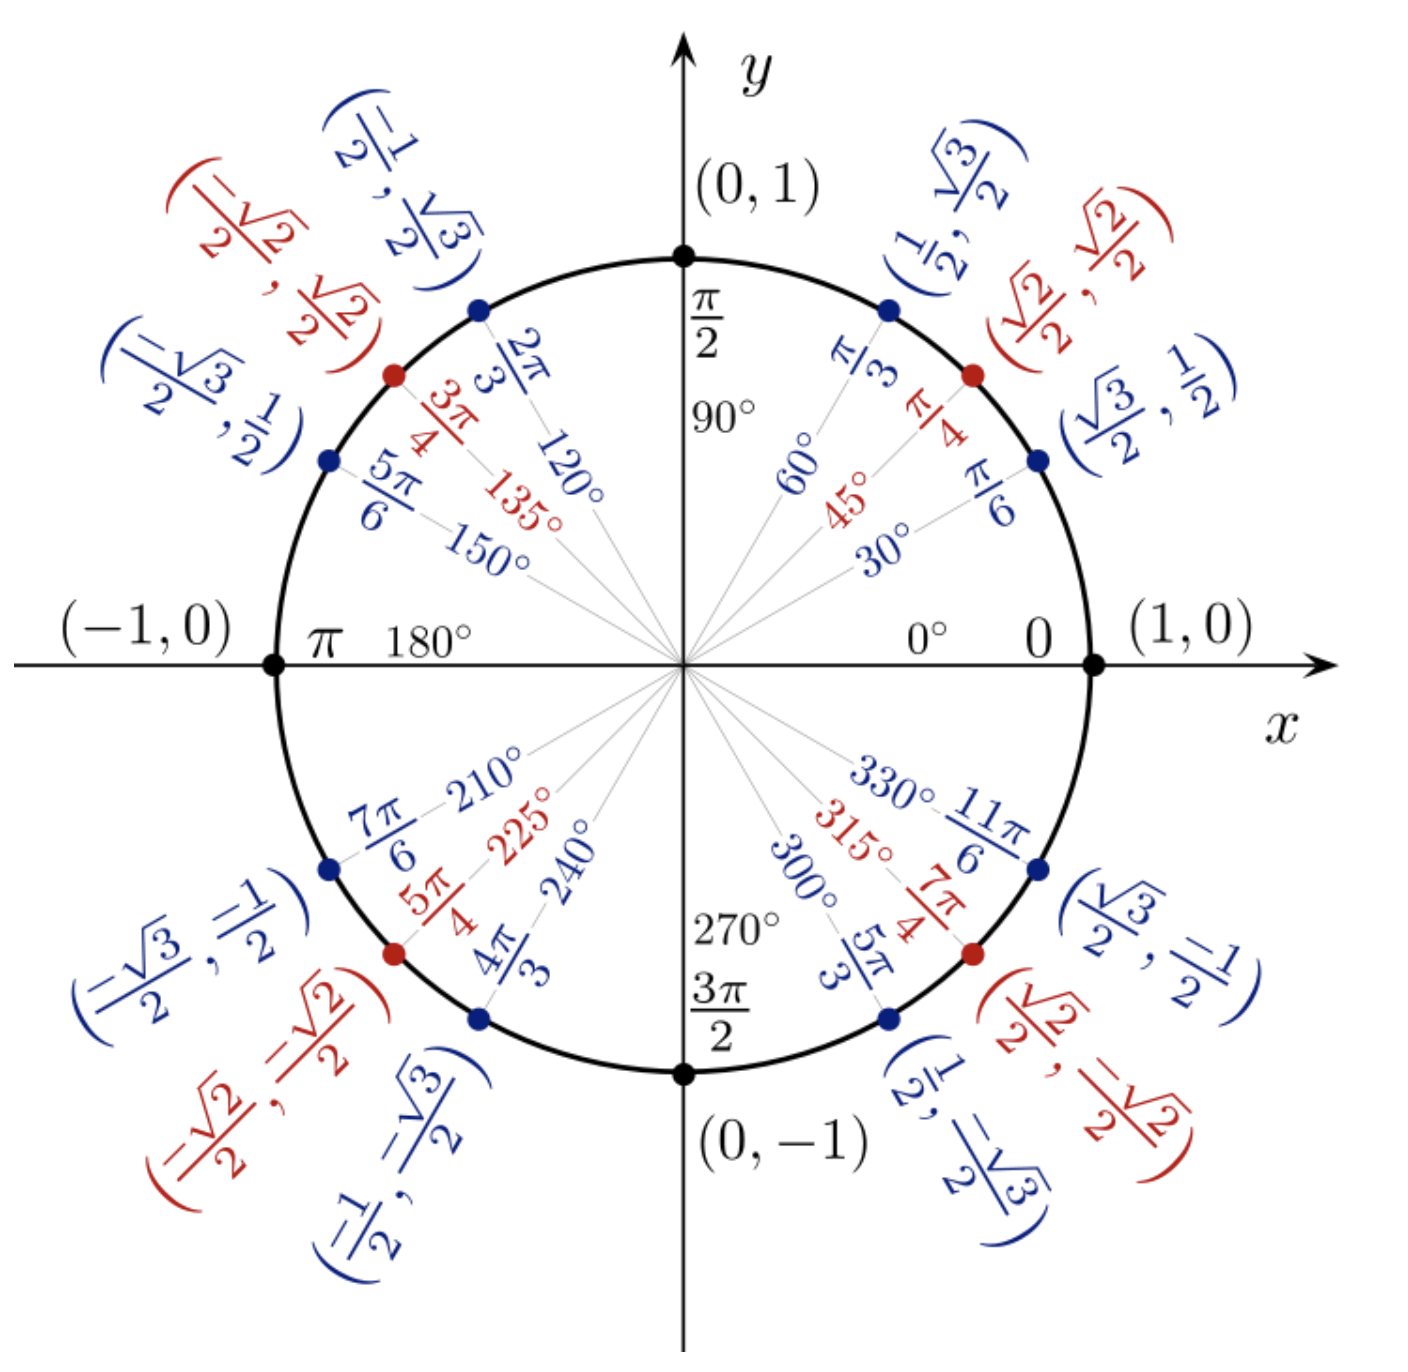
\includegraphics[width=0.5\linewidth]{Bilder/unit_circle.png}
    \caption{Unit Circle}
    \label{fig:unit_circle}
%Quelle : https://www.govst.edu/uploadedFiles/Academics/Colleges_and_Programs/CAS/Trigonometry_Short_Course_Tutorial_Lauren_Johnson.pdf%
\end{figure}
The following applies to all points that lie on the unit circle: 

\begin{equation}
    x^2 + y^2 = 1
\end{equation}

\subsubsection{Trigonometric Functions}

Trigonometric functions describe relationships between angles and side lengths in right-angled triangles. So we now consider right-angled triangles. The side opposite to the right-angle is called hypothenuse. If the length of the hypothenuse is called $c$ and the lengths of the two legs is given by $a$ and $b$, Pythagoras Theorem states that: 
\begin{equation}
    a^2+b^2=c^2.
\end{equation}
When considering an angle in a right triangle, the side of the triangle that touches the angle is called the adjacent side. The remaining third side is called opposite side. So, the length of hypothenuse, opposite and adjacent side define a right triangle. 
%Bild mit Hypothenuse, Gegen- und Ankathete, Bilder ähnlicherb Dreiecke%
We now consider similar right-angled triangles. Similar triangles have equal angles but different side lengths.
We now observe that the ratio of the side lengths is the same for similar triangles. So for a certain angle $\alpha $, the following fundamental ratios are defined. 
\begin{itemize}
    \item $\sin(\alpha) = \frac{\text{opposite}}{\text{hypotenuse}}$
    \item $\cos(\alpha) = \frac{\text{adjacent}}{\text{hypotenuse}}$
    \item $\tan(\alpha) = \frac{\text{opposite}}{\text{adjacent}}$
\end{itemize}
You can now also think of these equations as functions, where alpha is the variable. This means that, for a given angle, you are asking for the ratios of the side lengths of the corresponding right triangle. 
Trigonometric functions can be used to:
\begin{itemize}
    \item calculate missing side lengths
    \item determine unknown angles
\end{itemize}

To determine the values of $\sin(\alpha)$ and $\cos(\alpha)$ the unit circle can also be used. :

As you already komw, the  unit circle is a circle with radius $1$ centered at the origin. An angle $\alpha$ is measured from the positive x-axis and corresponds to a certain point on the unit circle. To find the corresponding point on the circle, imagine rotating a radius of length 1 by the angle $\theta$. The endpoint of this radius lies on the circle and has coordinates $(x,y)$.

This construction forms a right triangle:
\begin{itemize}
    \item the hypotenuse is the radius $r=1$
    \item the horizontal side has length $x$
    \item the vertical side has length $y$
\end{itemize}

Using the definitions of trigonometric functions in a right triangl, one obtains:
\begin{equation}
    \cos(\alpha) = \frac{\text{adjacent}}{\text{hypotenuse}} = x
\end{equation}
\begin{equation}
    \sin(\alpha) = \frac{\text{opposite}}{\text{hypotenuse}} = y
\end{equation}

Thus, the point on the unit circle corresponding to the angle $\alpha$ is described by the coordinates: $(\sin(\alpha), \cos(\alpha))$. 
So for $\alpha = 45^\circ$, the triangle is isosceles, so both legs are equal. Considering the unit circle, one can easily determine $\sin(\alpha)$ and $\cos(\alpha)$:
\begin{equation}
    \cos(45^\circ) = \sin(45^\circ) = \frac{\sqrt{2}}{2}
\end{equation}

\paragraph{Periodicity:}
The periodicity of sine and cosine function follows directly from the geometry of the unit circle. After a full rotation of $360^\circ$ (or $2\pi$ radians), the same  triangle is  created , and thus the point on the circle is identical. So, sine and cosine are periodic functions with a period of  $360^\circ$ (or $2\pi$ radians). 
In a more formal way, this is written as follows :
\begin{equation}
    \sin(\alpha + 2\pi) = \sin(\alpha), \quad \cos(\alpha + 2\pi) = \cos(\alpha)
\end{equation}

Another important identity is:
\begin{equation}
    \sin^2(x) + \cos^2(x) = 1
\end{equation}
This follows from the unit circle aswell. The right triangles that are considered show the side lengths of sine and cosine while the length of the hypothenuse is 1. Thus, the identity is derived using this characteristics and Pythagoras Theorem.  




\subsubsection{Graphs of Trigonometric Functions}

Trigonometric functions can also be represented graphically.
As we saw in the last section, sine and cosine function are periodic with a period of $2\pi$. 
\paragraph{Sine function}
%Bild einer Sinus-Fkt. einfügen%
When plotting the sine function we get to know more properties of it: 

\begin{itemize}
    \item \textbf{Domain \footnote{all possible input values (what you can plug into the function)}}: $(-\infty, \infty)$  
    This means you can insert any real number into the function.

    \item \textbf{Range \footnote{all possible output values (what comes out of the function)}}: $[-1,1]$  
    The output values of the sine function are always between $-1$ and $1$.

    \item \textbf{x-intercepts \footnote{points where the graph touches or crosses the x-axis}}: $x = n\pi$, where $n \in \mathbb{Z}$  
    These are the points where the graph crosses the x-axis (i.e., where $\sin(x)=0$).
    \item \textbf{Periodicity}:  
    The sine function repeats itself every $2\pi$:
    \begin{equation}
        \sin(x + 2\pi) = \sin(x)
    \end{equation}
    \item \textbf{Odd function}:  
    The sine function is symmetric with respect to the origin. This means:
    \begin{equation}
        \sin(-x) = -\sin(x)
    \end{equation}

\end{itemize}



\paragraph{Cosine Function}
%P=lot von Cosinus einfügen %
When plotting the cosine function one observes similar properties:

\begin{itemize}
    \item \textbf{Domain}: $(-\infty, \infty)$  
    Any real number can be used as input.

    \item \textbf{Range}: $[-1,1]$  
    The values always stay between $-1$ and $1$.

    \item \textbf{Periodicity}:  
    The cosine function also repeats every $2\pi$:
    \begin{equation}
        \cos(x + 2\pi) = \cos(x)
    \end{equation}
    \item \textbf{Even function}:  
    The cosine function is symmetric with respect to the y-axis. This means:
    \begin{equation}
        \cos(-x) = \cos(x)
    \end{equation}

\end{itemize}

\paragraph{Explanation of Even and Odd Functions:}
\begin{itemize}
    \item \textbf{Even function}: The graph looks the same on the left and right side (mirror symmetry at the y-axis)
    \item \textbf{Odd function}: The graph looks the same after rotating it by $180^\circ$ around the origin
\end{itemize}
Both sine and cosine functions are periodic and oscillate between $-1$ and $1$. This makes them especially useful for describing waves and oscillations in physics.

\subsubsection{Transformations of Sine and Cosine Functions}

Sine and cosine functions can be modified using parameters. The general form of such a function is:

\begin{equation}
    f(x) = a \cdot \sin(bx + c) + d \quad \text{or} \quad f(x) = a \cdot \cos(bx + c) + d
\end{equation}

Each parameter changes the graph in a specific way:

\begin{itemize}
    \item \textbf{Amplitude ($a$):}  
    The amplitude describes how ``tall'' the wave is. It tells you the maximum distance from the middle line (equilibrium).
    \begin{itemize}
        \item $|a| > 1$: the graph is stretched (bigger peaks)
        \item $0 < |a| < 1$: the graph is compressed (smaller peaks)
        \item $a < 0$: the graph is reflected across the x-axis
    \end{itemize}

    \item \textbf{Period ($b$):}  
    The parameter $b$ changes how long one full wave lasts.
    The period $T$ is given by:
    \begin{equation}
        T = \frac{2\pi}{b}
    \end{equation}
    \begin{itemize}
        \item $b > 1$: the wave is compressed (repeats faster)
        \item $0 < b < 1$: the wave is stretched (repeats slower)
    \end{itemize}

    \item \textbf{Phase shift ($c$):}  
    The phase shift moves the graph left or right.
    \begin{equation}
        \text{shift} = -\frac{c}{b}
    \end{equation}
    \begin{itemize}
        \item shift to the right if $c < 0$
        \item shift to the left if $c > 0$
    \end{itemize}

    \item \textbf{Vertical shift ($d$):}  
    The parameter $d$ moves the whole graph up or down.
    \begin{itemize}
        \item $d > 0$: graph shifts upward
        \item $d < 0$: graph shifts downward
    \end{itemize}
\end{itemize}

\paragraph{How to think about it :}
\begin{itemize}
    \item The \textbf{amplitude} tells you how strong the oscillation is.
    \item The \textbf{period} tells you how long it takes until the wave repeats.
    \item The \textbf{phase shift} tells you where the wave starts.
    \item The \textbf{vertical shift} moves the whole wave up or down.
\end{itemize}

\subsubsection{Relationship Between Sine and Cosine}

The sine and cosine functions are closely related and can be transformed into each other by a simple horizontal shift. In fact, they describe the same type of oscillation, but start at different points.

The relationship is given by:
\begin{equation}
    \cos(x) = \sin\left(x + \frac{\pi}{2}\right)
\end{equation}
\begin{equation}
    \sin(x) = \cos\left(x - \frac{\pi}{2}\right)
\end{equation}

This means that the cosine function is just the sine function shifted to the left by $\frac{\pi}{2}$ (a quarter of a full period), and vice versa.

\paragraph{How to think about it :}
\begin{itemize}
    \item Both functions describe the same wave shape.
    \item The only difference is where the wave starts.
    \item A shift of $\frac{\pi}{2}$ moves the starting point from a maximum (cosine) to a zero crossing (sine).
\end{itemize}

\paragraph{Summary:}
By changing the parameters $a$, $b$, $c$, and $d$, we can model many different types of waves and oscillations. This is especially important in physics, for example when describing sound waves or vibrations.


\subsection{Exponential Functions and Logarithms}

Exponential functions and logarithms play a central role in mathematics and physics. They are especially important when describing processes that grow or decay over time, such as sound intensity, population growth, or radioactive decay.

\subsubsection{Exponential Functions}

Exponential functions describe processes in which a quantity changes by a constant \textbf{percentage} rather than a constant amount. This is a key difference from linear functions. This means: the bigger the quantity already is, the faster it grows (or decays).

A linear function changes by adding the same amount each step:
\begin{equation}
    y = mx + b
\end{equation}

An exponential function changes by multiplying with the same factor each step:
\begin{equation}
    f(x) = a \cdot b^x
\end{equation}

\begin{itemize}
    \item $a$: initial value (starting amount)
    \item $b$: growth factor (multiplication factor per step)
\end{itemize}

\paragraph{Growth Factor and Percent Change}

The growth factor $b$ describes how much a quantity changes per step:
\begin{itemize}
    \item $b > 1$: exponential growth ($f(x)$ increases with increasing $x$ )
    \item $0 < b < 1$: exponential decay ($f(x)$ decreases with increasing $x$ )
\end{itemize}

\paragraph{Graphs of Exponential Functions}
%Plots von E-Funktionen einfügen%
When considering the graph of an exponential function one observes the following properties:

\begin{itemize}
    \item The graph is a smooth curve (not a straight line as e.g. a linear function)
    \item It is always above the x-axis (for $a > 0$)
    \item It has a \textbf{horizontal asymptote}
\end{itemize}

\paragraph{Horizontal Asymptote:} 
A horizontal asymptote is a line that the graph approaches but never reaches. Considering an exponential growth, the graph approches $y=0$ for $x \rightarrow -\infty$. So, with dexreasing $x$, the graph gets closer and closer to zero but never reaches the $x-$axis.



\paragraph{Long-Term Behavior}
\begin{itemize}
    \item For exponential growth ($b>1$): $f(x) \to \infty$ as $x \to \infty$, $f(x) \to 0$ as $x \to - \infty$, 
    \item For exponential  decay ($0<b<1$): $f(x) \to 0$ as $x \to \infty$ 
\end{itemize}

\paragraph{Euler's number $e$}
Euler's number, denoted as $e$, is one of the non-terminating constants we often use in mathematics and science. Another non-terminating constant you might already know is $\pi$ which is often used in geometry.
Euler’s number approximately equals 2.71828. You also obtain $e$ when calculating the following term for very large numbers $n$: 
\begin{align}
    e \approx  \left( 1+ \frac{1}{n} \right)^n
\end{align}
With increasing $n$ the term approches $e$ as you can see in the following table: 
\begin{table}[h]
\centering
\begin{tabular}{|c|c|}
\hline
$n$ & $\left(1 + \frac{1}{n}\right)^n$ \\
\hline
1      & 2{.}000000 \\
2      & 2{.}250000 \\
5      & 2{.}488320 \\
10     & 2{.}593742 \\
100    & 2{.}704814 \\
1000   & 2{.}716924 \\
10000  & 2{.}718146 \\
100000 & 2{.}718268 \\
\hline
$\infty$ & $e \approx 2{.}718282\ldots$ \\
\hline
\end{tabular}
\caption{approximation of Euler's number $e$ as $n$ increases}
\label{tab:euler}
\end{table}
Euler’s number helps mathematicians, physicists and other scientists explain exponential growth in various phenomena, from population to radioactive decay. So, euler's number $e$ often becomes the growth factor when describing natural phenomena. The following function is thus very important in math and physics: 
\begin{align}
    f(x) = a \cdot e^x
\end{align}




\paragraph{Transformations of Exponential Functions}

Similar to sine and cosine functions, exponential functions can also be changed using different parameters. These parameters allow us to adjust the shape and position of the graph.

The general form is:
\begin{equation}
    f(x) = a \cdot b^{k(x-c)} + d
\end{equation}

Each parameter has a clear effect on the graph:

\begin{itemize}
    \item \textbf{Parameter $a$ (vertical scaling):}  
    This parameter stretches or compresses the graph vertically.
    \begin{itemize}
        \item $a > 1$: the graph becomes steeper (grows faster visually)
        \item $0 < a < 1$: the graph becomes flatter
        \item $a < 0$: the graph is flipped upside down (reflection at the x-axis)
    \end{itemize}

    \item \textbf{Parameter $k$ (growth speed):}  
    This parameter controls how fast the function grows or decays.
    \begin{itemize}
        \item larger $k$: faster growth or decay
        \item smaller $k$: slower change
    \end{itemize}
    You can think of $k$ as controlling how ``quickly'' the curve rises or falls.

    \item \textbf{Parameter $c$ (horizontal shift):}  
    This moves the graph left or right.
    \begin{itemize}
        \item shift to the right if $c > 0$
        \item shift to the left if $c < 0$
    \end{itemize}
    This means the function starts growing earlier or later.

    \item \textbf{Parameter $d$ (vertical shift):}  
    This moves the entire graph up or down.
    \begin{itemize}
        \item $d > 0$: graph moves up
        \item $d < 0$: graph moves down
    \end{itemize}
\end{itemize}


By changing these parameters, we can adapt exponential functions to model many real-world processes, such as population growth or decay processes in physics.


\subsubsection{Logarithms}

The logarithm is the inverse operation of an exponential function. While an exponential function answers the question

\begin{center}
    \textit{``What is the result if we raise a number to a certain power?''}
\end{center}

the logarithm answers the reverse question:

\begin{center}
    \textit{``To which power must we raise a number to obtain a given result?''}
\end{center}

Mathematically, this relationship is written as:
\begin{equation}
    b^x = y \quad \Longleftrightarrow \quad \log_b(y) = x
\end{equation}

Here:
\begin{itemize}
    \item $b$ is the base
    \item $x$ is the exponent
    \item $y$ is the result
\end{itemize}

\paragraph{Example:}
\begin{equation}
    2^3 = 8 \quad \Longleftrightarrow \quad \log_2(8) = 3
\end{equation}

\paragraph{Intuitive Explanation:}
\begin{itemize}
    \item Exponential function: you start with a number and calculate the result
    \item Logarithm: you are given the result and want to find the exponent
\end{itemize}

\paragraph{Important Notes:}
\begin{itemize}
    \item Logarithms are only defined for positive numbers ($y > 0$)
    \item The base must be positive and not equal to 1
\end{itemize}

\paragraph{Summary:}
The logarithm is a tool that helps us ``undo'' exponential growth. It is especially useful when we want to solve equations where the unknown is in the exponent.


\subsubsection{Natural Logarithm}

The logarithm with base $e$ is called the natural logarithm and denoted by $\ln$:
\begin{equation}
     log_e (y) = \ln(y)
\end{equation}


So the natural logarithm answers the question:
\begin{center}
    \textit{``To which power must we raise $e$ to get a certain number?''}
\end{center}


\paragraph{Inverse Relationship}

Exponential and logarithmic functions undo each other:
\begin{equation}
    e^{\ln(x)} = x
\end{equation}
\begin{equation}
    \ln(e^x) = x
\end{equation}

%Plots von ln und e-Fkt einfügen%

From the graphs, we can also see that the natural logarithm function and the exponential function cancel each other out. This means they are \textbf{inverse functions}.

Geometrically, this relationship can be observed by the fact that their graphs are mirror images of each other along the line
\begin{equation}
    y = x
\end{equation}
which is also called the angle bisector.

\paragraph{Intuitive Explanation:}
\begin{itemize}
    \item The exponential function $e^x$ takes an input $x$ and produces a value
    \item The logarithm $\ln(x)$ takes this value and returns the original input $x$
\end{itemize}

So applying one function after the other brings you back to where you started:
\begin{equation}
    \ln(e^x) = x \quad \text{and} \quad e^{\ln(x)} = x
\end{equation}

\subsubsection{Summary}

\begin{itemize}
    \item Exponential functions describe growth and decay processes
    \item The number $e$ is fundamental for natural growth
    \item Logarithms are the inverse of exponential functions
    \item Both concepts are essential for modeling real-world phenomena
\end{itemize}


%%%%%%%%%%%%%%%%%%%%%%%%%%%%%%%%%%%%%%%%%%%%%%%%%%%%%%%%%%%%%%
